\begin{figure}[htb]
    \centering
    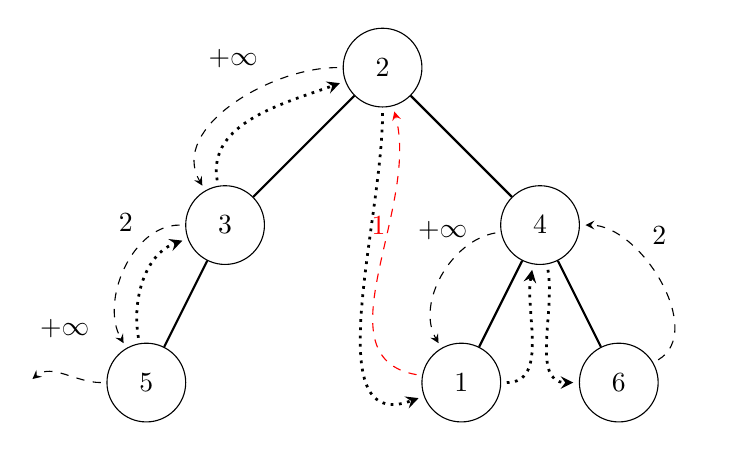
\begin{tikzpicture}[baseline=-2.25cm]
        \node[circle,draw,minimum size=1cm] (1) at (0,0)  {$2$};
        \node[circle,draw,minimum size=1cm] (2) at (-2,-2){$3$};
        \node[circle,draw,minimum size=1cm] (3) at (2,-2) {$4$};
        \node[circle,draw,minimum size=1cm] (4) at (-3,-4){$5$};
        \node[circle,draw,minimum size=1cm] (5) at (1,-4) {$1$};
        \node[circle,draw,minimum size=1cm] (6) at (3,-4) {$6$};
        % \node[label={7},circle,draw,minimum size=1cm] (7) at (3,-4) {$8$};
        % \node[label={8},circle,draw,minimum size=1cm] (8) at (-4,-6) {$4$};
        % \node[label={9},circle,draw,minimum size=1cm] (9) at (-2,-6) {$1$};
        \tikzstyle{filho}=[thick]
        \tikzstyle{pred}=[->, shorten >= 2pt, shorten <= 2pt, dashed, >=stealth]
        \tikzstyle{sucessor}=[->, shorten >= 2pt, shorten <= 2pt, dotted, >=stealth, line width=0.35mm]
        % \tikzstyle{p4}=[->, shorten >= 2pt, shorten <= 2pt, dotted, >=stealth]
        \draw[filho] (1) -- (2);
        \draw[filho] (1) -- (3);
        \draw[filho] (2) -- (4);
        \draw[filho] (3) -- (5);
        \draw[filho] (3) -- (6);
        \draw[pred] (6) edge[out=30,in=0]
        node[above=10pt] {$2$} (3);
        \draw[sucessor] (3) edge[out=280,in=180] (6);
        \draw[pred] (3) edge[out=190,in=120]
        node[above=10pt] {$+\infty$} (5);
        \draw[sucessor] (5) edge[out=0,in=260] (3);
        \draw[pred, red] (5) edge[out=170,in=285]
        node[red, above=10pt] {$1$} (1);
        \draw[sucessor] (1) edge[out=270,in=200] (5);
        \draw[pred] (1) edge[out=180,in=120]
        node[above=10pt] {$+\infty$} (2);
        \draw[sucessor] (2) edge[out=100,in=200] (1);
        \draw[pred] (2) edge[out=180,in=120]
        node[above=10pt] {$2$} (4);
        \draw[sucessor] (4) edge[out=100,in=200] (2);
        \draw[pred] (4) edge[out=180,in=40]
        node[above=10pt] {$+\infty$} (-4.5, -4);
    \end{tikzpicture}
    \begin{tabular}{|c|c|c|c|c|}
        \hline
        &       &       & $\now = 0$ & $\now = 1$ \\
        $i$ & $x_0$ & $v$   & $\cert[i]$ & $\cert[i]$ \\
        \hline
        $1$ & $6$   & $2$   & $1$        & $+\infty$  \\
        $2$ & $3$   & $5$   & $+\infty$  & $+\infty$  \\
        $3$ & $2$   & $1$   & $2$        & $2$        \\
        $4$ & $7$   & $4$   & $+\infty$  & $4$        \\
        $5$ & $-2$  & $3$   & $+\infty$  & $+\infty$  \\
        $6$ & $14$  & $0.5$ & $2$        & $2$        \\
        \hline
    \end{tabular}
    \caption[Representação de certificado expirado]{Certificado do
    elemento $1$ expirou em $\now = 1$.}\label{fig:abb:expire}
\end{figure}